\documentclass[a4paper,12pt]{article}
\usepackage[utf8]{inputenc}
\usepackage{amsmath, amssymb, amsthm}
\usepackage{graphicx}
\usepackage{hyperref}
\usepackage{fancyhdr}
\usepackage{xcolor}
\usepackage{geometry}
\usepackage{titling}
\usepackage{enumitem}
\usepackage{longtable}

\geometry{top=2cm, bottom=2cm, left=2.5cm, right=2.5cm}

\hypersetup{
    colorlinks=true,
    linkcolor=black,
    filecolor=magenta,      
    urlcolor=cyan,
    pdftitle={Simulación de Exploración y Recolección Planetaria con Robots},
    pdfpagemode=FullScreen,
}

\pagestyle{fancy}
\fancyhf{}
\lhead{Simulación Planetaria con Robots}
\rhead{Inteligencia Artificial}
\cfoot{\thepage}
\renewcommand{\contentsname}{Contenidos}

\title{
    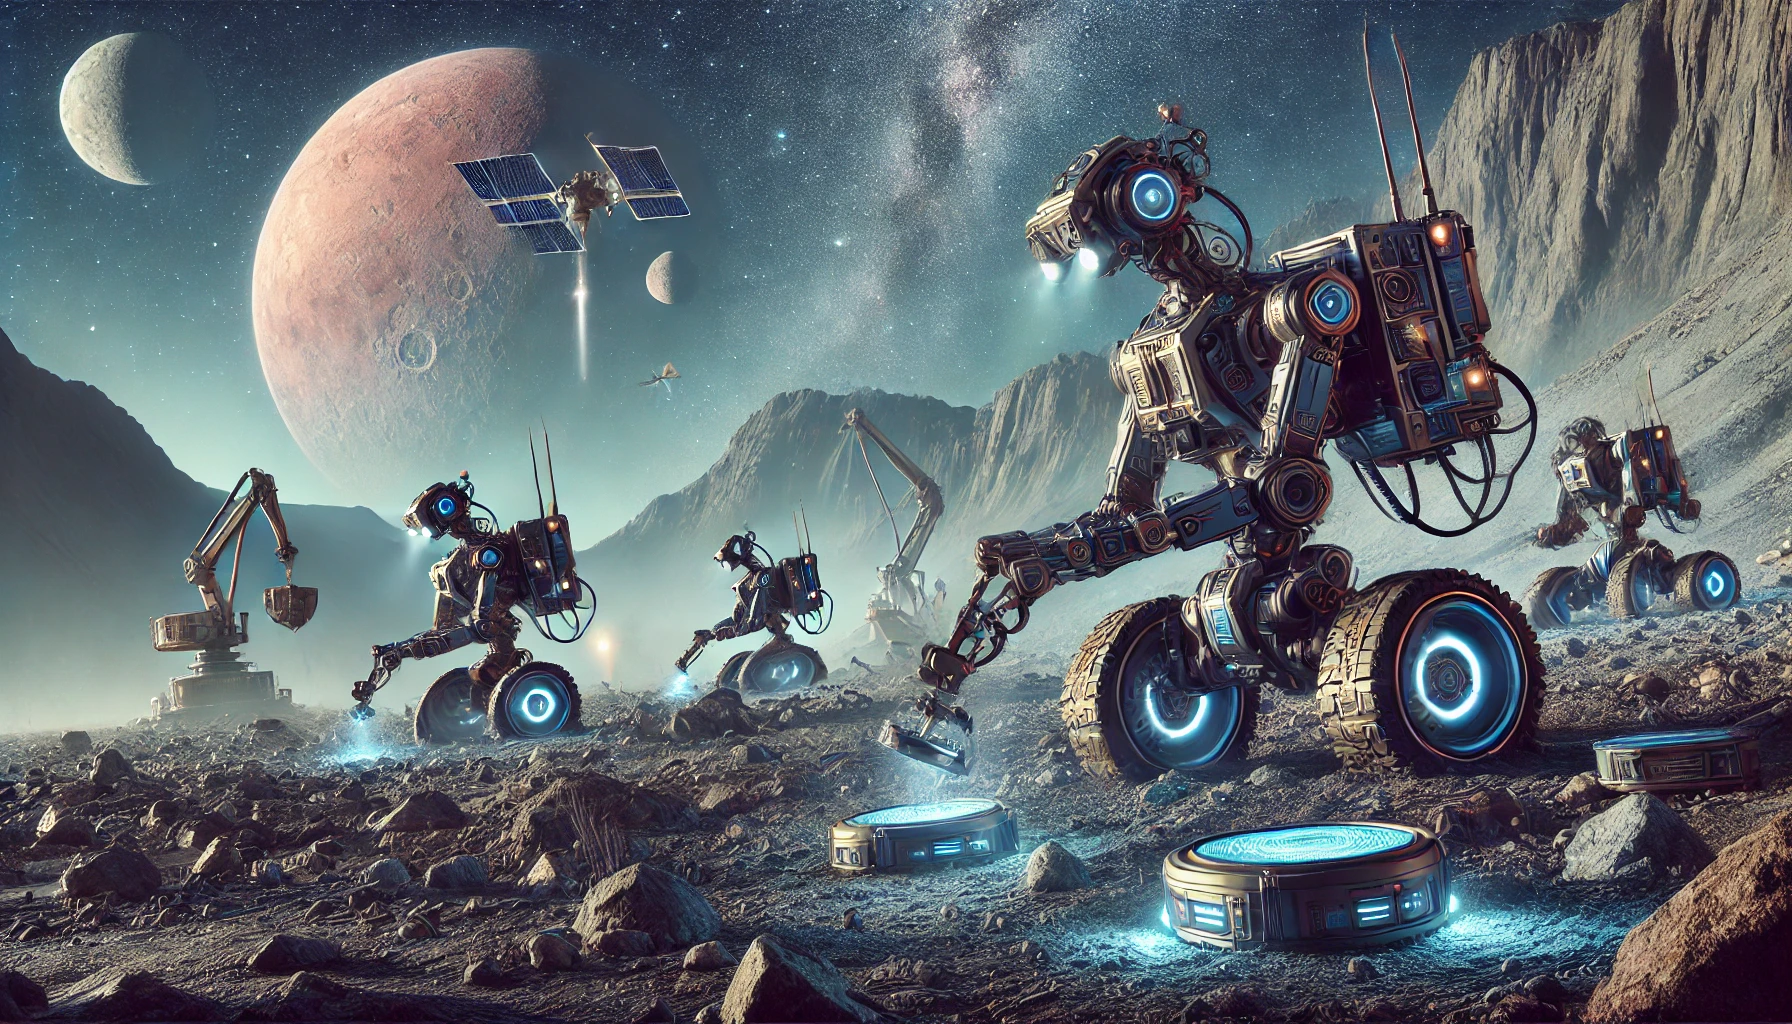
\includegraphics[width=1\textwidth]{images/portada.jpg} \\ 
    \vspace{3cm}
    \textbf{Simulación de Exploración y Recolección Planetaria con Robots}\\[0.5cm]
}
\author{Íñigo Martínez Jiménez}
\date{}


\begin{document}

\maketitle



\newpage
\section*{Introducción}
En esta documentación he elaborado una explicacion sobre el diseño e implementación de una simulación orientada a la exploración y recolección en un planeta  mediante robots autónomos. Los robots, divididos en exploradores y recolectores, trabajan en conjunto para descubrir ecosistemas y recolectar recursos, con la finalidad de construir una base en el planeta y a partir de esta, lograr una optimización de estos. El objetivo principal es poder minimizar el tiempo de construcción de la base en el planeta, teniendo en cuenta la cantidad de robots que se utilizan así como el tamaño del planeta.\\\\

Se detallan las entidades, eventos y procesos involucrados, así como estructura del código, los diagramas de clases y paquetes, los algoritmos evolutivos y la parte de inteligencia que de la cual se ha dotado al proyecto. Además, se presenta un flujo de trabajo que facilitan la comprensión de la simulación.\\\\ 
\tableofcontents
\newpage


\section{Estructura del Código}
El código está desarrollado en la carpeta \texttt{CODIGO}, con las siguientes subcarpetas y archivos:
\begin{itemize}[label=\textbullet]
    \item \textbf{ANÁLISIS:}
    \begin{itemize}[label=\textendash]
        \item \texttt{analysis.ipynb}: Fichero con el análisis del producto cartesiano con las distintas combinaciones de nuestros parámetros del algoritmo evolutivo.
        \item \texttt{pso.py}: Fichero con la implementación del algoritmo evolutivo así como la función fitness y el producto cartesiano.
        \item \texttt{dataframe.csv}: Fichero .csv donde se almacenan los resultados del producto cartesiano.
        \item \texttt{\_\_init\_\_py}: Inicializador del módulo.
    \end{itemize}
    \item \textbf{ENTIDADES:}
    \begin{itemize}[label=\textendash]
        \item \texttt{base.py}: Fichero con la clase correspondiente a la base del planeta.
        \item \texttt{ecosystem.py}: Fichero con la clase correspondiente a los ecosistemas del planeta.
        \item \texttt{planet.py}: Fichero con la clase correspondiente al planeta.
        \item \texttt{robot.py}: Fichero con las clases correspondientes a los robots explorador y recolector.
        \item \texttt{\_\_init\_\_py}: Inicializador del módulo.
    \end{itemize}
    \item \textbf{EVENTOS:}
    \begin{itemize}[label=\textendash]
        \item \texttt{events.py}: Fichero engargado de la gestión de eventos del planeta.
        \item \texttt{\_\_init\_\_py}: Inicializador del módulo.
    \end{itemize}
    \item \textbf{OP FUZZY MARKOV:}
    \begin{itemize}[label=\textendash]
        \item \texttt{fuzzy.py}: Fichero con la implementación de la lógica difusa para tomar la decisión de si los robots deben volver a la base.
        \item \texttt{operations.py}: Fichero donde se desarrollan metodos para calcular operaciones como la distancia Manhattan o la normalización de un número.
        \item \texttt{weather\_markov.py}: Fichero donde se desarrolla el modelo Markoviano que modela y predice el tiempo en el planeta durante la simulación.
        \item \texttt{\_\_init\_\_py}: Inicializador del módulo.
    \end{itemize}
    \item \textbf{PROCESOS:}
    \begin{itemize}[label=\textendash]
        \item \texttt{processes.py}: Fichero que ejecutan los procesos de recolectar y explorar de los robots.
        \item \texttt{\_\_init\_\_py}: Inicializador del módulo.
    \end{itemize}
    \item \textbf{VIRT\_ENV:}
    \begin{itemize}[label=\textendash]
        \item \texttt{Lib}: Entorno virtual del proyecto donde se almacenan todas las librerías que se han utilizado en el código.
    \end{itemize}
    \item \texttt{app.py}: Implementación principal de la simulación.
    \item \texttt{requierments.txt}: Fichero \texttt{.txt} que contiene todas librerías necesarias para que el código funcione correctamente.
\end{itemize}

\section{Diagrama de paquetes}
    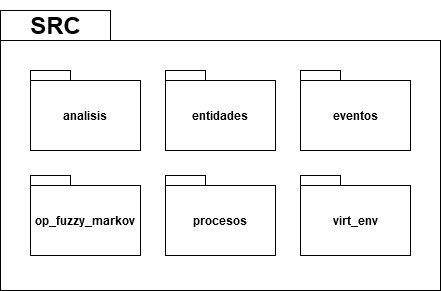
\includegraphics[scale=1]{images/diag_paquetes.png}

\section{Representación del planeta}
La base siempre se sitúa siempre en el centro del planeta. Los diferentes ecosistemas están repartidos aleatoriamente alrededor de la base, siendo el número de estos un \texttt{20\%} de las casillas. 

\begin{center}
    \centering
    \begin{tabular}{|c|c|c|c|c|c|c|c|c|c|c|} \hline 
         E1&  ..&    ..&  ..&  ..&  ..&  ..&  ..&   ..& ..&..\\ \hline 
         ..&  ..&    ..&  ..&  ..&  ..&  ..&  ..&   E7& ..&..\\ \hline 
         ..&  ..&    ..&  E2&  ..&  ..&  ..&  ..&   ..& ..&..\\ \hline 
         ..&  ..&  ..&  ..&  ..&  ..&  ..&  ..&   ..& ..&  ..\\ \hline 
         ..&  ..&  ..&  ..&  ..&  ..&  ..&  E4&   ..& ..&..\\ \hline 
         ..&  E3&  ..&  ..&  ..&  B&  ..&  ..&   ..& ..&..\\ \hline 
         ..&  ..&  ..&  ..&  ..&  ..&  ..&  ..&   ..& ..&..\\ \hline 
         ..&  ..&  ..&  ..&  ..&  ..&  ..&  ..&   E5& ..&..\\ \hline 
         .&  ..&  ..&  E6&  ..&  ..&  ..&  ..&   ..& ..&..\\ \hline 
         .&  ..&  ..&  ..&  ..&  ..&  ..&  ..&   ..& E8&..\\ \hline 
        E9& ..& ..& ..& ..& ..& ..& ..& ..& ..&..\\ \hline
    \end{tabular}

    \label{tab:my_label}
\end{center}

\newpage    
\section{Descripción del Sistema}
\subsection{Componentes de la simulación}
\subsubsection{Entidades}
\begin{itemize}[label=\textbullet]
    \item \textbf{Robot Explorador(Robot)}: Es una clase heredada de la clase Robot, y su objetivo es explorar el planeta con la finalidad de encontrar ecosistemas. Se mueve gracias al método \texttt{move()}, el cual le permite moverse en cuatro direcciones [North, South, East, West].
    \item \textbf{Robot Recolector(Robot)}: Al igual que el robot explorador, es una clase heredada de la clase Robot, su objetivo es recolectar recursos así como comprobar si la base está lista para construir. Por otro lado, lleva implementado un sistema de deción basado en la lógica difusa para decidir si él y su pareja exploradora deben volver a la base a recargar.
    \item \textbf{Planeta}: Es una rejilla bidimensional, la cual contiene una cantidad finita de ecosistemas y gestiona sus estados. Este planeta se genera aleatoriamente al principio de cada simulación posicionando aleatoriamente también los ecosistemas en distintas ubicaciones.
    \item \textbf{Ecosistema}: Representa las áreas del planeta con materiales, más concretamente agua y minerales. Estos poseen un atributo llamado \texttt{dificultad}, el cual afectará a la energía de los robots.
    \item \textbf{Base}: Administra los materiales recolectados utilizando su propio sistema autónomo para construirse, además, posee una estación de carga donde los robots recuperan su batería.\\\\
\end{itemize}
\subsubsection{Procesos}
\begin{itemize}[label=\textbullet]
    \item \textbf{Proceso clima}: Es el proceso encargado de manejar el clima del planeta en la simulación. Gracias al método \texttt{planet\_weather()}, el cual hace uso de un modelo Markoviano, hemos podido modelar el clima de manera que vaya cambiando cada 20 segundos. 
    \item \textbf{Proceso explorar}: Al igual que el robot explorador, es una clase heredada de la clase Robot, su objetivo es recolectar recursos así como comprobar si la base está lista para construir. Por otro lado, lleva implementado un sistema de deción basado en la lógica difusa para decidir si él y su pareja exploradora deben volver a la base a recargar.
    \item \textbf{Proceso recolectar}: Es una clase heredada de la clase Robot, y su objetivo es explorar el planeta con la finalidad de encontrar ecosistemas. Se mueve gracias al método \texttt{move()}, el cual le permite moverse en cuatro direcciones [North, South, East, West].   
\end{itemize}
\newpage
\subsubsection{Eventos}
\begin{itemize}[label=\textbullet]
    \item \textbf{Evento ecosistema encontrado}: Ocurre cuando un robot explorador se encuentra en una casilla del mapa en donde hay un ecosistema, y este se lo reporta a su recolector para que acuda a recolectarlo.
    \item \textbf{Evento recolección de ecosistema}: Ocurre cuando un robot recolector llega al ecosistema para recolectarlo, una vez terminado decide si volver a la base en función de la disponibilidad de su capacidad.    
\end{itemize}

\subsection{Diagrama de Clases}

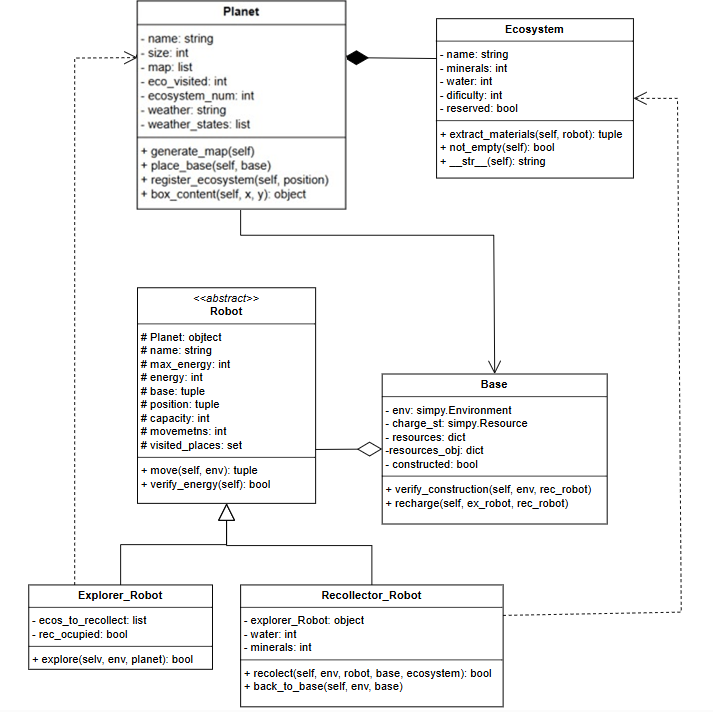
\includegraphics[scale=0.85]{images/diag_clases.png}


\newpage

\subsection{Flujo del Proceso}

Todos los robots comienzan en la base la cual está siempre ubicada en el centro del mapa. Cada explorador, está asociado a un recolector, por lo que estos últimos estarán en la base esperando hasta que su explorador les reporte algún ecosistema.
\\\\
Los exploradores comienzan a moverse de manera aleatoria buscando ecosistemas, y en el momento en el que encuentrar uno, reportan ese ecosistema al recolector, que se dirige hacia él para recolectarlo. En el caso de que ese ecosistema ya haya sido visitado por algún otro robot, este robot seguirá explorando sin reportárselo a su recolector. Cuando un explorador encuentra un ecosistema, este lo reserva para que nigún otro robot pueda arrebatárselo.
\\\\
El recolector empieza a extraer los recursos mientras el explorador se queda esperando hasta que reciba la señal del reoclector de que ha finalizado su tarea. Una vez ha llenado su capacidad, vuelve a la base para almacenar los recursos. Una vez en la base, hace una consulta al explorador para saber si quedan recursos en el ecosistema, si es así, vuelve para recolectarlos, en caso contrario, mandaría la señal de que su explorador puede continuar con su exploración y se quedaría en la base esperando a que este encontrase otro ecosistema. Si el robot recolector extrajese todos los recursos de un ecosistema sin llenar su capacidad, no volvería a la base y se quedaría esperando en el ecosistema a que su explorador reportase otro ecosistema. 
\\\\
La energía de los robots se irá consumiendo en función de las actividades que vayan realizando durante la simulación y dependiendo del clima que haya en el planeta. Exploradores y recolectores consumirán su energía cada vez que se mueven, así como cada vez que interctuán con un ecosistema, disminuyendo esta en función de la dificultad que presente. Los diferentes tipos de clima (clear, stormy, tornado) afectarán significativamente a la energía de cada robot cada vez que realicen alguna actividad.
\\\\
A partir de la lógica difusa implementada, si alguno de los dos robots recibe un aviso sobre su energía, ambos vuelven a la base para recargar y una vez finalizada su recarga, vuelven a empezar de nuevo sus respectivas funciones.
\\\\

\section{Simulación}
La simulación mide el tiempo de cada acción en días. La simulación se finaliza en dos circunstancias, la primera, cuando todos los recursos necesarios se han recolectado y por lo tanto la base se ha construido, y la segunda, si todos los ecosistemas del planeta ya se han explorado y no ha recursos suficientes para construir la base, por lo que el planeta quedaría descartado.
\\\\
Cada acción que va realizando cada uno de los robots en la simulación se especifica en el el output del código indicando el tiempo en de la simulación en el momento en el que se realiza la acción, la energía restante del robot, el tipo de robot, el número de identificación del robot. En el caso de que sea un robot explorador se mostrará también la posición a la que se mueve, y si es un reoclector, se indicará los recursos que ha recolectado.

\section{Implementación de lógica difusa}
Dado que la decisión de volver a cargar a la base no siempre se podía determinar a partir de una única regla, se implementa un sistema difuso que produce un valor estimado que representa la decisión de volver a la base o no.
\\\\
A partir de tres variables [\texttt{energy, distance, decision}], siendo esta última la variable respuesta, podemos determinar la decisión del robot, estableciendo funciones de pertenencia para cada una de las variables y evaluandolas cada una de ellas con los inputs [\texttt{energy, distance}] en las reglas difusas. De este modo, creamos un sistema de control el cual se basa en las siguientes condiciones:
\begin{enumerate}
    \item \textbf{Regla 1:} Si la energía es \textit{muy baja} (\texttt{very\_low}) y la distancia es \textit{cercana} (\texttt{close}), entonces la decisión es \textit{volver a la base} (\texttt{return}).
    \item \textbf{Regla 2:} Si la energía es \textit{muy baja} (\texttt{very\_low}) y la distancia es \textit{lejana} (\texttt{far}), entonces la decisión es \textit{volver a la base} (\texttt{return}).
    \item \textbf{Regla 3:} Si la energía es \textit{baja} (\texttt{low}) y la distancia es \textit{cercana} (\texttt{close}), entonces la decisión es \textit{continuar} (\texttt{continue}).
    \item \textbf{Regla 4:} Si la energía es \textit{baja} (\texttt{low}) y la distancia es \textit{lejana} (\texttt{far}), entonces la decisión es \textit{volver a la base} (\texttt{return}).
    \item \textbf{Regla 5:} Si la energía es \textit{alta} (\texttt{high}) y la distancia es \textit{cercana} (\texttt{close}), entonces la decisión es \textit{continuar} (\texttt{continue}).
    \item \textbf{Regla 6:} Si la energía es \textit{alta} (\texttt{high}) y la distancia es \textit{lejana} (\texttt{far}), entonces la decisión es \textit{continuar} (\texttt{continue}).
\end{enumerate}

\section{Implementación del Modelo de Markov}
A partir de una matriz de transición, se ha sido capaz de modelar el clima del planeta de la simulación, consiguiendo así predecir el clima que hará en el planeta cada 20 unidades de tiempo. A continuación, se muestra una representación gráfica de la cadena de Markov utilizada:

\begin{center}
    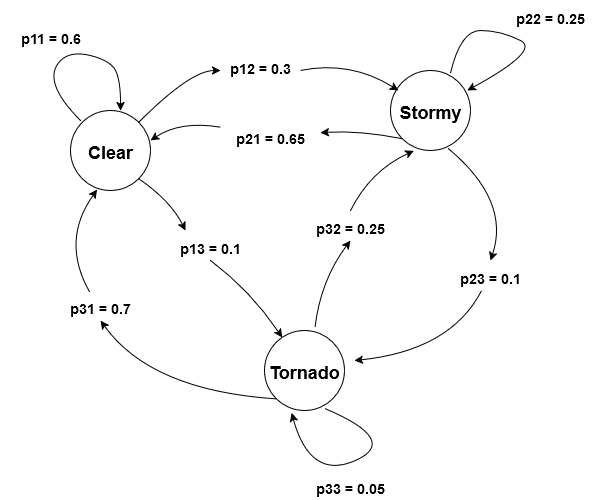
\includegraphics[scale=0.48]{images/Markov_Chain.png}
\end{center}

\newpage
\section{Implementación de algoritmo evolutivo}
Dado que el objetivo principal es poder minimizar el tiempo de construcción de la base en el planeta, hemos implementado un algortimo evolutivo por enjambre de partículas(PSO), importado directamente desde la librería \texttt{Pyswarm}, y bastante eficaz si hablamos en términos de optimización.
\\\\
Para ello, se desarrolla una función fitness que mejor se adapte a lo que queremos optimizar. Esta función fitness evaluará la calidad de la solución teniendo en cuenta que nuestras variables dependientes serán el tiempo de construción(\texttt{time}), el número de robots(\texttt{num\_robots}) y el coste asociado de los robots(\texttt{cost}). Además, habrá una alta penalización a las combinaciones que no logren construir la base, pudiendo así descartarlas para centrarnos mejor en nuestro óptimo global. Nuestra función fitness está definida como:\\\\
\begin{equation}
f(x) = t + \left(\frac{C_\text{max}}{C}\right) \cdot 2 + n \cdot 0.3 + P
\end{equation}

Donde: 
\begin{itemize}
    \item $f(x)$: Valor de fitness.
    \item $t$: Unidades de tiempo necesarias para completar la construcción.
    \item $C$: Costo total asociado de los robots, calculado como $C = n \cdot 8$, donde $n$ es el número de parejas de robots.
    \item $C_\text{max}$: Costo máximo, calculado como $C_\text{max} = n_\text{max} \cdot 8$, donde $n_\text{max}$ es el número máximo de parejas de robots.
    \item $P$: Penalización aplicada si la construcción no se completa:
    \[
    P =
    \begin{cases} 
    10,000,000 & \text{si no se completa la base}, \\
    0 & \text{en caso contrario}.
    \end{cases}
    \]
\end{itemize}

Una vez implementado el PSO, se realiza un producto cartesiano con las distintas combinaciones que pueden encontrar sus parámetros, pudiendo así explorar de manera más concisa nuestro espacio de soluciones. Los resultados de este producto cartesiano, se almacenaran en un \texttt{.csv} para posteriormente analizarlos y sacar conclusiones. Ese fichero tendra el nombre de \texttt{dataframe.csv}, el cual contiene las siguientes columnas:

\begin{itemize}
    \item \textbf{particles:} Número de partículas en el enjambre.
    \item \textbf{omega:} Coeficiente de inercia.
    \item \textbf{phip:} Coeficiente de aceleración cognitiva.
    \item \textbf{phig:} Coeficiente de aceleración social.
    \item \textbf{max\_iter:} Número máximo de iteraciones.
    \item \textbf{Best solution:} Mejor solución encontrada por el PSO.
    \item \textbf{Fitness value:} Valor de fitness asociado a la mejor solución.
\end{itemize}
\end{document}